%% Informe breve de avance del proyecto TRI (formato IEEEtran, español).
%% Compilar: pdflatex -> bibtex -> pdflatex -> pdflatex
\documentclass[10pt,journal]{IEEEtran}

\usepackage[T1]{fontenc}
\usepackage[utf8]{inputenc}
\usepackage[spanish,es-noshorthands,es-tabla]{babel}
\usepackage{amsmath,amssymb}
\usepackage{graphicx}
\usepackage{booktabs}
\usepackage{array}
\usepackage{tikz}
\usetikzlibrary{arrows.meta,positioning}
\usepackage{url}
\usepackage[hidelinks]{hyperref}
\usepackage{cite}

\renewcommand{\IEEEkeywordsname}{Palabras clave}

\begin{document}

\title{Proyecto Tri: informe de avance sobre la localización de objetos dentro de una cavidad metálica con señales Wi-Fi}

\author{Juan~David~Quijano~B., Samuel~David~Luna~Ortega, Santiago~Alejandro~Narváez~Coral,
        Nicolás~Díaz~Palomares, Esteban~Felipe~Rincón~Alvarado
        y~Andrés~Felipe~Soler~Guevara (grupo ingesaurios)%
\thanks{Los autores pertenecen a la Facultad de Ingeniería de Datos e Inteligencia Artificial, Universidad Santo Tomás, Colombia.}%
\thanks{Informe de avance, noviembre de 2026.}}

\markboth{Informe de avance del proyecto Tri, noviembre de 2026}%
{Quijano \MakeLowercase{\textit{et al.}}: Informe de avance del proyecto Tri}

\maketitle

\begin{abstract}
Tri (Triceraptor) estudia si la información del estado del canal Wi-Fi (CSI) que registran placas comerciales de bajo costo permite saber en qué posición está un objeto dentro de una caja metálica cerrada, sin cámaras y sin colocar ningún sensor sobre el objeto. Este informe resume el estado del proyecto en noviembre de 2026. El montaje físico ya funciona: un router doméstico emite dentro de una caja de zinc y cuatro receptores ESP32-S3 graban la señal mientras un cilindro de agua salada se cuelga en las posiciones de una malla tridimensional. La recolección de datos está en curso, con una meta inicial de casi 500 datos etiquetados. En paralelo se construyó la cadena de procesamiento, desde la verificación automática de cada toma hasta la evaluación de los modelos. El preprocesamiento de las tomas se paralelizó con \texttt{multiprocessing} de Python y, en un procesador de 8 núcleos, se ejecuta 5,8 veces más rápido que la versión secuencial con resultados idénticos. Se compararon cuatro enfoques de reconocimiento. Por ahora el más sencillo, que busca la posición ya medida más parecida, iguala o supera a las redes neuronales probadas. Los resultados son preliminares. El trabajo que queda se concentra en repetir mediciones de las mismas posiciones, controlar los cambios de la señal entre días y calibrar el criterio con el que el sistema declara una posición como desconocida.
\end{abstract}

\begin{IEEEkeywords}
CSI Wi-Fi, localización pasiva, cavidad metálica, ESP32-S3, reconocimiento de posiciones.
\end{IEEEkeywords}

\section{Introducción}
\IEEEPARstart{C}{uando} una señal Wi-Fi viaja de un emisor a un receptor, cada objeto en el camino la refleja o la absorbe un poco. La tarjeta de red mide ese efecto en cada una de las subportadoras de la transmisión, y ese registro se llama información del estado del canal (CSI, por sus siglas en inglés). Desde que existen herramientas para leer la CSI en tarjetas comerciales \cite{halperin2011tool}, se ha usado para detectar personas, gestos y actividades \cite{ma2019wifi}, y para localizar a una persona en una sala sin que lleve ningún dispositivo \cite{xiao2013pilot,dang2019device}. Hoy también se puede leer en microcontroladores baratos como el ESP32 \cite{hernandez2020lightweight}.

Casi todos esos trabajos buscan personas en habitaciones grandes, con errores del orden de un metro. Tri plantea otro escenario: un objeto pequeño e inmóvil dentro de una caja metálica cerrada. En una cavidad así la señal rebota muchas veces en las paredes, y esos rebotes hacen que la huella de la señal cambie mucho con desplazamientos pequeños. Experimentos de física con equipos de laboratorio mostraron que esa riqueza de rebotes sirve para localizar con mucha resolución \cite{delhougne2021deeply}. La pregunta de Tri es si se puede aprovechar con hardware comercial de pocos dólares.

El informe está organizado así. La Sección~\ref{sec:problema} plantea el problema y su relación con los Objetivos de Desarrollo Sostenible (ODS), y la Sección~\ref{sec:objetivos} fija los objetivos. Las Secciones~\ref{sec:montaje} y~\ref{sec:recoleccion} describen el montaje y la recolección de datos. La Sección~\ref{sec:modelos} presenta los modelos en desarrollo y la Sección~\ref{sec:paralelo}, el módulo de preprocesamiento paralelo con su reporte de rendimiento. La Sección~\ref{sec:integracion} explica qué aportan las asignaturas de Redes e infraestructura y de Analítica y visualización de datos. Las Secciones~\ref{sec:estado} a~\ref{sec:conclusiones} resumen el estado actual, las dificultades, los próximos pasos y las conclusiones.

\section{Planteamiento del problema}\label{sec:problema}
Saber dónde está un objeto dentro de un espacio cerrado suele exigir una cámara, que necesita luz y línea de vista y registra imágenes, o un sensor pegado al objeto. La CSI ofrece una alternativa pasiva, porque el objeto altera la señal sin llevar nada encima. Pero la literatura de sensado Wi-Fi casi no ha estudiado recintos metálicos cerrados con hardware comercial \cite{ma2019wifi}, y no se sabe si en ellos la huella de la señal es lo bastante estable para reconocer posiciones de un día a otro. Esa es la pregunta científica de Tri.

El proyecto tiene además un problema de cómputo. Cada toma debe preprocesarse antes de llegar a los modelos, y la cadena actual lo hace una toma tras otra. Con la meta de casi 500 tomas, y con cada cambio en el preprocesamiento obligando a repetirlo todo, ese paso secuencial alarga cada ciclo de prueba del modelado. La Sección~\ref{sec:paralelo} aborda ese cuello de botella.

El trabajo se relaciona con dos ODS de la Agenda 2030 \cite{onu2015agenda}. El más directo es el ODS~9 (industria, innovación e infraestructura), cuya meta~9.5 pide aumentar la investigación científica y la capacidad tecnológica de los países en desarrollo. Tri hace investigación experimental en Colombia con un router doméstico y placas ESP32-S3 en lugar de los analizadores de redes de laboratorio que usan los trabajos de física sobre cavidades \cite{delhougne2021deeply}, lo que abarata repetir y ampliar el experimento. El segundo es el ODS~3 (salud y bienestar), a más largo plazo: un sensado sin cámaras y sin contacto podría servir para vigilar signos en personas sin registrar imágenes. Hoy Tri trabaja solo con un objeto inerte, y cualquier prueba con personas necesitará aval ético.

\section{Objetivos}\label{sec:objetivos}
El objetivo general es determinar si la CSI Wi-Fi captada con hardware comercial de bajo costo permite reconocer en qué posición se encuentra un objeto dentro de una cavidad metálica cerrada. Los objetivos específicos son:
\begin{enumerate}
    \item montar la cavidad con un router comercial, cuatro receptores ESP32-S3 y un sistema de captura sincronizada;
    \item construir un conjunto de datos etiquetado sobre una malla de posiciones, con referencias de caja vacía;
    \item medir qué tan estable es la señal al quitar y volver a colocar el objeto, al moverlo pocos centímetros y de un día a otro;
    \item comparar métodos de reconocimiento, desde el vecino más cercano hasta redes neuronales, con una evaluación que no mezcle datos de entrenamiento y de prueba;
    \item reconocer también la caja vacía y las posiciones que el sistema nunca ha visto.
\end{enumerate}

El planteamiento cambió respecto al resumen presentado en la Feria de la Ciencia. Aquella versión usaba una jaula de aluminio y buscaba estimar las coordenadas $(x,y)$ del objeto con una red convolucional. Las primeras mediciones mostraron que la señal dentro de la cavidad cambia demasiado rápido para interpolar entre posiciones, de modo que el problema se replanteó como reconocer posiciones conocidas de una malla 3D.

\section{Montaje experimental}\label{sec:montaje}
La cavidad es una caja cerrada de zinc de $100 \times 100 \times 70$~cm. Dentro, un router TP-Link Archer C50 transmite en la banda de 2,4~GHz y cuatro placas ESP32-S3, una en cada pared y con antena externa, registran la CSI de cada trama que reciben. Una Raspberry Pi concentra los cuatro flujos, los alinea y los guarda.

El objeto de prueba es un cilindro con agua salada de 9,5~cm de diámetro y 11~cm de alto. El agua salada se comporta ante la señal de forma parecida al cuerpo humano, y el cilindro es inerte, así que se puede colgar en cualquier punto todas las veces que haga falta. Las posiciones forman una malla de $10 \times 10$ puntos en planta, separados 8~cm, repetida a cuatro alturas. A cada celda de esa malla la llamamos \emph{boxel}.

\section{Recolección de datos}\label{sec:recoleccion}
La captura la guía una página web servida por la Raspberry Pi. El operador ve qué posición toca, cuelga el cilindro, cierra la caja e inicia la grabación de una toma de varios segundos. Al terminar, la toma sube sola a Google Drive con su etiqueta de posición y sus metadatos. Con la misma rutina se graban tomas de caja vacía, que sirven de referencia, y tomas de validación en las que el cilindro se vuelve a colgar en una posición ya medida.

La meta inicial del conjunto de datos es de casi 500 datos, donde cada dato es una toma etiquetada. La Fig.~\ref{fig:flujo} muestra el recorrido de los datos desde la caja hasta los modelos.

\begin{figure}[!t]
\centering
\begin{tikzpicture}[
    caja/.style={draw, rounded corners=2pt, align=center, font=\footnotesize,
                 minimum height=0.9cm, text width=1.55cm},
    flecha/.style={-{Latex[length=2mm]}, thick}]
\node[caja] (cav) {Cavidad\\router y\\4 ESP32-S3};
\node[caja, right=0.35cm of cav] (pi) {Raspberry Pi\\captura y\\etiquetado};
\node[caja, right=0.35cm of pi] (drive) {Google\\Drive};
\node[caja, right=0.35cm of drive] (mod) {Verificación\\y modelos};
\draw[flecha] (cav) -- (pi);
\draw[flecha] (pi) -- (drive);
\draw[flecha] (drive) -- (mod);
\end{tikzpicture}
\caption{Flujo de los datos en Tri. La recolección y el modelado van por separado: el modelado solo lee de Drive y trabaja con una copia local.}
\label{fig:flujo}
\end{figure}

Antes de que una toma llegue a los modelos, un programa revisa que esté completa y que su etiqueta sea coherente. Las tomas defectuosas o mal etiquetadas se excluyen. Después se corrige el ajuste automático de ganancia de cada receptor, se resume la toma en un perfil por nodo y se compara con una toma de caja vacía grabada en el mismo estado del montaje. Esa comparación importa porque la caja cambia un poco de un día a otro (al abrirla y cerrarla, por ejemplo), y sin ella el sistema confundiría esos cambios con el objeto.

En la recolección no participan personas ni animales y no se registran datos personales; el único sujeto es el cilindro. Si en el futuro se trabaja con personas, habrá que tramitar el consentimiento informado y el aval del comité de ética correspondiente.

\section{Modelos en desarrollo}\label{sec:modelos}
Todos los modelos reciben lo mismo: la CSI de los cuatro nodos mientras el cilindro está en una posición. La Tabla~\ref{tab:modelos} resume qué hace cada uno y en qué estado está.

\begin{table}[!t]
\renewcommand{\arraystretch}{1.2}
\caption{Modelos evaluados en Tri}
\label{tab:modelos}
\centering
\footnotesize
\begin{tabular}{@{}>{\raggedright\arraybackslash}p{2.1cm}>{\raggedright\arraybackslash}p{3.2cm}>{\raggedright\arraybackslash}p{2.1cm}@{}}
\toprule
Modelo & Qué hace & Estado \\
\midrule
Vecino más cercano & Busca la posición ya medida con la huella más parecida; también responde ``caja vacía'' o ``desconocido'' & Modelo oficial \\
Red de prototipos con atención & Parte del vecino más cercano y aprende a corregir la huella & Empata con el oficial; se retomará con más datos \\
CavityVoxel-Former & Transformer que da la probabilidad de cada boxel & Quedó por debajo; se guarda como referencia \\
Regresión de posición & Intenta estimar coordenadas de puntos no medidos & Exploratorio; confirmó que no se puede interpolar \\
\bottomrule
\end{tabular}
\end{table}

El modelo oficial compara la huella de una toma nueva con una galería de huellas de posiciones ya medidas. La huella combina la forma de la señal a lo largo de las subportadoras y el nivel de señal de cada nodo. Si la toma no se parece lo bastante a nada conocido, el sistema la marca como desconocida en lugar de forzar una respuesta.

El proyecto empezó con CavityVoxel-Former, un transformer diseñado para reconstruir el volumen de la caja. Con los datos disponibles quedó por debajo del vecino más cercano, y lo mismo pasó con otras redes probadas. Por eso se decidió que una red solo reemplaza al método simple si lo supera de forma clara en la misma evaluación. Esa evaluación separa siempre las tomas de entrenamiento y de prueba, porque mezclarlas infla los aciertos, un problema ya documentado en sensado Wi-Fi \cite{varga2024mitigating}.

Ya hay métricas cuantitativas preliminares. El sistema reconoce posiciones ya vistas después de retirar y volver a colgar el cilindro, distingue la caja vacía y suele rechazar las posiciones que no conoce. Una prueba posterior con tomas nuevas confirmó el comportamiento del modelo oficial. Todavía hay pocas repeticiones por posición, así que las cifras tienen márgenes amplios y no se reportan en este informe.

El hallazgo negativo también cuenta. Con la malla de 8~cm, la señal de una posición no se puede predecir a partir de sus vecinas, porque cambia demasiado en pocos centímetros. Tri puede reconocer posiciones medidas, pero no adivinar las intermedias.

El código está en Python (PyTorch, NumPy, SciPy y scikit-learn), tiene pruebas automáticas y se publica en el repositorio del proyecto en GitHub. Los entrenamientos se ejecutan en una GPU de escritorio.

\section{Módulo de preprocesamiento paralelo}\label{sec:paralelo}
Preprocesar una toma significa leer su CSV comprimido, alinear los cuatro nodos por el número de secuencia de cada trama, normalizar la amplitud, calcular la fase diferencial y resumir la toma en un perfil medio por nodo. La cadena del proyecto hace esto con la función \texttt{tramas\_de} del repositorio \texttt{cavityvoxel-former}, una toma detrás de otra. Ninguna toma depende de otra, así que el problema admite paralelismo de datos: cada trabajador recibe tomas completas y devuelve solo su perfil, una matriz de $4 \times 52$ valores, para que la comunicación entre procesos sea mínima.

El módulo \texttt{tri\_paralelo.py} reparte las tomas con \texttt{multiprocessing.Pool} (\texttt{map} con \texttt{chunksize=1}, para equilibrar la carga) y llama a la misma función del proyecto sin modificarla. Para comparar, también ejecuta la versión secuencial y una versión con \texttt{ThreadPoolExecutor}. Se midió el tiempo de pared sobre un lote fijo de 64 tomas, con tres repeticiones por configuración, y se tomó la mediana. Ese tiempo incluye crear y cerrar el \emph{pool}, que en Windows arranca cada proceso desde cero. Con $T_1$ como tiempo secuencial y $T_p$ como tiempo con $p$ trabajadores, el speedup y la eficiencia son
\begin{equation}
S_p = \frac{T_1}{T_p}, \qquad E_p = \frac{S_p}{p}.
\end{equation}
Las pruebas se hicieron en un AMD Ryzen 7 PRO 4750G (8 núcleos físicos, 16 hilos) con Windows 11, Python 3.13 y NumPy 2.4. En todas las configuraciones el módulo comprueba que los perfiles calculados en paralelo son idénticos, bit a bit, a los secuenciales, y lo fueron. El código, las instrucciones para repetir la medición y los resultados en CSV están en la carpeta \texttt{modulo\_paralelo}.

\begin{table}[!t]
\renewcommand{\arraystretch}{1.15}
\caption{Rendimiento del preprocesamiento de 64 tomas ($T_1 = 38{,}90$~s)}
\label{tab:rendimiento}
\centering
\footnotesize
\begin{tabular}{@{}rrrrrrr@{}}
\toprule
 & \multicolumn{3}{c}{\texttt{multiprocessing}} & \multicolumn{3}{c}{\texttt{threading}} \\
\cmidrule(lr){2-4}\cmidrule(l){5-7}
$p$ & $T_p$ (s) & $S_p$ & $E_p$ & $T_p$ (s) & $S_p$ & $E_p$ \\
\midrule
1  & 37,99 & 1,02 & 1,02 & 37,40 & 1,04 & 1,04 \\
2  & 19,83 & 1,96 & 0,98 & 36,85 & 1,06 & 0,53 \\
4  & 10,49 & 3,71 & 0,93 & 35,86 & 1,08 & 0,27 \\
8  &  6,70 & 5,81 & 0,73 & 37,73 & 1,03 & 0,13 \\
12 &  6,39 & 6,08 & 0,51 & 38,86 & 1,00 & 0,08 \\
16 &  6,21 & 6,26 & 0,39 & 39,63 & 0,98 & 0,06 \\
\bottomrule
\end{tabular}
\end{table}

\begin{figure*}[!t]
\centering
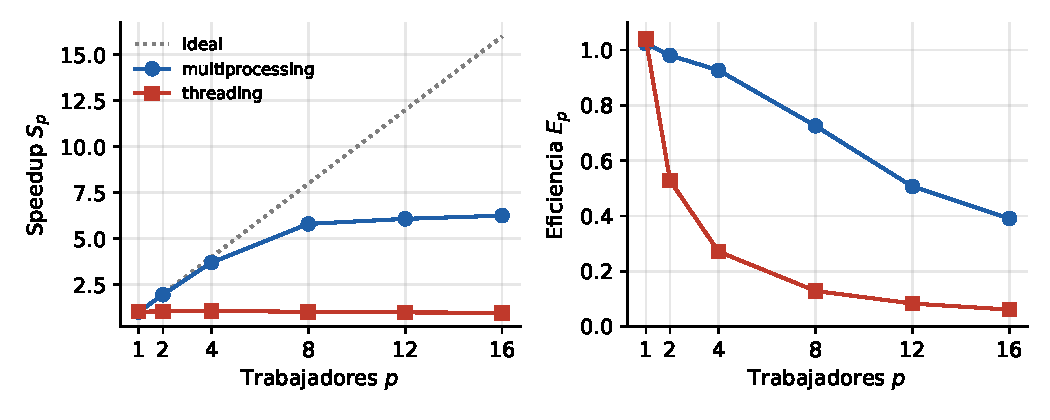
\includegraphics[width=0.82\textwidth]{modulo_paralelo/resultados/speedup_eficiencia.pdf}
\caption{Speedup (izquierda) y eficiencia (derecha) del preprocesamiento paralelo frente al número de trabajadores. La línea punteada es el speedup ideal $S_p = p$.}
\label{fig:speedup}
\end{figure*}

La Tabla~\ref{tab:rendimiento} y la Fig.~\ref{fig:speedup} muestran los resultados. Con procesos, el speedup es casi lineal hasta cuatro trabajadores ($E_4 = 0{,}93$) y llega a 5,81 con ocho, de modo que el preprocesamiento tarda 6,7~s en lugar de 38,9~s. Pasar de 8 a 16 procesos solo sube el speedup de 5,81 a 6,26. El procesador tiene 8 núcleos físicos; los 8 hilos adicionales comparten las unidades de cálculo de esos núcleos y aportan poco a una tarea que ocupa la CPU todo el tiempo. La métrica de Karp--Flatt, $e = (1/S_p - 1/p)/(1 - 1/p)$, apunta en la misma dirección: vale 0,019 con dos procesos, 0,054 con ocho y 0,104 con dieciséis. Si el límite fuera solo una parte secuencial fija del programa, $e$ se mantendría constante; que crezca con $p$ indica un costo que aumenta con el número de procesos, como el arranque de cada uno y la competencia por los núcleos y el disco.

Con hilos no hay mejora: el speedup se queda alrededor de 1 con cualquier número de hilos. La lectura del CSV se hace en Python puro, y el bloqueo global del intérprete (GIL) de CPython deja que un solo hilo ejecute código Python a la vez. Para esta tarea, por tanto, hay que usar procesos. El valor de $S_1$ ligeramente mayor que 1 se debe a la variación entre repeticiones, del orden del 2~\%.

Con base en estas medidas, para el uso normal se recomiendan ocho procesos, que dan casi todo el speedup disponible con una eficiencia de 0,73. El código de recolección y la cadena del proyecto no se modificaron. Si el equipo lo aprueba, el siguiente paso es ofrecer el modo paralelo como opción de la cadena de preprocesamiento, una vez comprobado que da los mismos archivos que la versión actual.

\section{Integración con otras asignaturas}\label{sec:integracion}
Dos asignaturas de cuarto semestre aportan componentes que ya funcionan en Tri.

\emph{Redes e infraestructura.} La captura depende de una red pequeña que el equipo configuró y mantiene. Las cuatro placas ESP32-S3 envían cada medición por Wi-Fi a la Raspberry Pi en paquetes UDP de 279 bytes con una cabecera propia, y la Pi los recibe en un puerto fijo. UDP encaja con este uso: cada nodo envía decenas de paquetes por segundo, perder alguno es aceptable y esperar retransmisiones, como haría TCP, retrasaría la grabación. Antes de grabar, la Pi espera a que los cuatro nodos sostengan al menos 50 paquetes por segundo durante 3~s, y anula la sesión si alguno se cae. Como cada placa tiene su propio reloj, la Pi ajusta un modelo de desfase y deriva por nodo para poner todas las mediciones en una base de tiempo común. La Pi se conecta por Ethernet al router de salida a Internet; por esa vía sube cada toma a Google Drive con \texttt{rclone} y sirve la página web de captura en la red local.

\emph{Analítica y visualización de datos.} Cada toma pasa por un análisis de calidad antes de usarse: un script genera el inventario de tomas, la lista de tomas aptas, la de tomas por repetir y un informe con la repetibilidad entre tomas de la misma posición, la información que aporta cada nodo y la cobertura de la malla. La página de captura muestra al operador qué posición toca, el tiempo grabado y una estimación de lo que falta. Los resultados de los modelos se resumen con intervalos de confianza y pruebas estadísticas, y el reporte de rendimiento de la Sección~\ref{sec:paralelo} se presenta con la tabla y la gráfica de speedup y eficiencia. El ecosistema de repositorios del proyecto incluye además un visor 3D de los boxeles en vivo (\texttt{voxel-viewer}).

\section{Estado actual}\label{sec:estado}
La Tabla~\ref{tab:estado} reúne lo terminado y lo que está en curso.

\begin{table}[!t]
\renewcommand{\arraystretch}{1.2}
\caption{Estado de las actividades del proyecto}
\label{tab:estado}
\centering
\footnotesize
\begin{tabular}{@{}>{\raggedright\arraybackslash}p{5.6cm}l@{}}
\toprule
Actividad & Estado \\
\midrule
Montaje de la cavidad y captura con cuatro nodos & Terminado \\
Pilotos de calibración del montaje & Terminado \\
Cadena de datos: descarga, verificación e índice & Terminado \\
Revisión del estado del arte & Terminado \\
Modelo oficial con caja vacía y rechazo & Terminado \\
Protocolo de evaluación sin fuga de datos & Terminado \\
Prueba con datos nuevos & Terminado \\
Módulo de preprocesamiento paralelo & Terminado \\
Recolección por la malla y de validación & En curso \\
Repeticiones de las mismas posiciones & En curso \\
Calibración del umbral de ``desconocido'' & En curso \\
Artículo científico & Por iniciar \\
\bottomrule
\end{tabular}
\end{table}

Uno de los pilotos se descartó porque una pieza de presión en la tapa alteraba la señal. Ese tropiezo dejó una regla de trabajo: cualquier cambio físico en la caja se anota, porque la señal lo registra.

\section{Dificultades y próximos pasos}\label{sec:dificultades}
La dificultad principal es que la caja cambia de estado entre sesiones. Abrirla, cerrarla o mover un cable produce saltos en la señal de la caja vacía que pueden ser tan grandes como la diferencia entre dos posiciones. A eso se suma que volver a colgar el cilindro nunca lo deja exactamente igual. Con pocas repeticiones por posición, ninguna red neuronal tiene datos suficientes para superar al método simple.

Los próximos pasos responden a esas dificultades:
\begin{enumerate}
    \item grabar varias veces las mismas posiciones, retirando y recolocando el cilindro, que es lo que más limita hoy;
    \item anotar el estado del montaje en todas las tomas y grabar una caja vacía cada cierto tiempo;
    \item calibrar el umbral con el que el sistema declara una posición como desconocida;
    \item hacer una prueba con puntos intermedios entre celdas para cerrar la pregunta de la interpolación;
    \item probar más ancho de banda o saltos entre canales, para obtener más información por toma;
    \item escribir el artículo y preparar la publicación del conjunto de datos.
\end{enumerate}

Hay también un riesgo operativo: la autorización de Google Drive en la Raspberry Pi vence cada cierto tiempo, y si no se renueva las tomas dejan de subir.

\section{Conclusiones}\label{sec:conclusiones}
Tri ya tiene un montaje que funciona, una rutina de recolección que etiqueta y sube cada toma sin intervención manual, y una cadena de evaluación que separa los datos de entrenamiento y de prueba. Los primeros resultados indican que la huella Wi-Fi dentro de la caja metálica basta para reconocer posiciones ya medidas y para distinguir la caja vacía. También muestran un límite claro: con una malla de 8~cm no se puede predecir lo que pasa entre puntos. En la parte de cómputo, el preprocesamiento paralelo con ocho procesos es 5,8 veces más rápido que el secuencial y da los mismos resultados, lo que acorta cada ciclo de prueba del modelado. La prioridad del siguiente periodo es medir más veces las mismas posiciones y registrar el estado de la caja. Con esos datos se podrá saber si las redes neuronales aportan algo sobre el método simple y cuánta confianza merecen los resultados.

\bibliographystyle{IEEEtran}
\bibliography{referencias_informe_tri}

\end{document}
